\begin{Propriete}[Variations du trinôme]
    Soit $f$ une fonction définie sur $\mathbb{R}$ par $f(x) = ax^{2} + bx + c$ une fonction polynôme du second degré ($a \neq 0$) avec forme canonique $f(x) = a(x-\alpha)^{2} + \beta$.
    
    Les variations du trinôme $f$ sont données par les tableaux suivants :
    
    \begin{tcbenumerate}
        \tcbitem Si $a > 0$, la fonction $f$ est décroissante sur l'intervalle $\CrochetD-\infty;\alpha\CrochetD$ et croissante sur l'intervalle $\CrochetG\alpha ; +\infty\CrochetG$.
        
        \begin{center}
        \begin{tabular}{cc}
        \begin{tikzpicture}[scale=0.7]
            %Fonction    
            \draw[line width=1.2pt,color=monrose,smooth,samples=100,domain=-0.8:2.6] plot(\x,{0.8*(\x-1)^(2.0)+1})node [above] {$\mathcal{P}$};    
            % Point
            \draw[blue,very thick,dashed,-] (0,1) node[left] {\large{$\beta$}} -- (1,1) -- (1,0) node[below] {\large{$\alpha$}};   
            %Tangente
            \draw[blue,thick,<->] (0.5,1) -- (1.5,1);    
            % Axes
            \draw[thick,->] (-1.5,0) -- (3.5,0);
            \draw[thick,->] (0,-0.5) -- (0,4);
        \end{tikzpicture}
        &
        \begin{tikzpicture}
        \tkzTabInit{$x$/1,$f$/1.8}
        {$-\infty$,$\alpha$,$+\infty$}
        \tkzTabVar{+/$+\infty$,-/$\beta$,+/$+\infty$}
        \end{tikzpicture}
        \end{tabular}
        \end{center}
        
        \tcbitem Si $a < 0$, la fonction $f$ est croissante sur l'intervalle $\CrochetD-\infty;\alpha\CrochetD$ et décroissante sur l'intervalle $\CrochetG\alpha ; +\infty\CrochetG$.
        
        \begin{center}
        \begin{tabular}{cc}
        \begin{tikzpicture}[scale=0.7]
            %Fonction    
            \draw[line width=1.2pt,color=monrose,smooth,samples=100,domain=-0.8:2.6] plot(\x,{-0.8*(\x-1)^(2.0)+3})node [below] {$\mathcal{P}$};    
            % Point
            \draw[blue,very thick,dashed,-] (0,3) node[left] {\large{$\beta$}} -- (1,3) -- (1,0) node[below] {\large{$\alpha$}};   
            %Tangente
            \draw[blue,thick,<->] (0.5,3) -- (1.5,3);
            % Axes
            \draw[thick,->] (-1.5,0) -- (3.5,0);
            \draw[thick,->] (0,-0.5) -- (0,4);
        \end{tikzpicture}
        &
        \begin{tikzpicture}
        \tkzTabInit{$x$/1,$f$/1.8}
        {$-\infty$,$\alpha$,$+\infty$}
        \tkzTabVar{-/$-\infty$,+/$\beta$,-/$-\infty$}
        \end{tikzpicture}
        \end{tabular}
        \end{center}
    \end{tcbenumerate}
\end{Propriete}